\newpage

\section{Opis przeprowadzonych badań}

\subsection{Sieci Bayesowskie}

\subsection{Ukryte modele Markowa}

Badania dla ukrytego modelu Markowa przeprowadzono dla zobrazowania podstawowych zależności zachodzących między zbiorem podstawowym nie posiadającym żadnej wiedzy o problemie, czy w tym wypadku chorobie, oraz zbioru sekwencyjnego, taką wiedzę posiadającą. Ideą zbioru sekwencyjnego było aby składał się on z danych wskazujących w jaki sposób zmieniała się choroba wraz z czasem.

W projekcie wykorzystano zbiór charakteryzujący problem raka piersi z darmowego internetowego zasobu \textit{UCI}, który to nie posiadał historii choroby\footnote{Link do zbioru: \url{https://archive.ics.uci.edu/ml/datasets/Breast+Cancer}}. Należało zatem historię przemian wygenerować własnoręcznie. Posłużono się w tym celu macierzą przejść łańcucha Markowa, który przedstawiał prawdopodobieństwa przejścia od klasy \textit{X} do klasy \textit{Y}, bądź zostania dalej w klasie \textit{X}. Cały schemat generowania sekwencji przedstawić można w kilku krokach:
\\
\begin{enumerate}
  \item Stwórz macierz przejść łańcucha Markowa
  \item Posortuj próbki po klasie
  \item Dla każdej próbki:
    \begin{enumerate}
    \item Wybierz następną klasę z prawdopodobieństwem z macierzy
    \item Dla wybranej klasy wybierz próbkę z prawdopodobieństwem losowym
    \item Dopisz wybraną klasę i próbkę jako sekwencja
    \end{enumerate}
\end{enumerate}

\par
\bigskip

Posiadając oba zbioru - bazowy oraz sekwencyjny, przeprowadzono badania najważniejszych parametrów modelu - czasu uczenia, czasu testowania oraz efektywności. Manipulowano przy tym dostępnym parametrem - algorytmem dekodowania, gdzie starano się zbadać jaki wpływ na wyniki ma zmiana algorytmu. Zastosowano dwa algorytmy - algorytm Viterbiego bazujący na technice programowania dynamicznego, oraz algorytm heurystyczny "best-first" znany także jako algorytm dekodowania posteriori.

Jako stałe parametry przyjęto długość sekwencji na 2, gdyż wstępne badania wykazały, iż zwiększenie sekwencji nie wpływa w zauważalny sposób na wyniki. Niezmienny był także współczynnik zbioru testowego, wynoszący 0.2, co wskazywało, iż 20\% zbioru wejściowego wykorzystywane jest jako zbiór testowy. Następnym niezmiennym parametrem był parametr wejściowy do algorytmu - alfa, który to w literaturze angielskiej określany jest jako \textit{Lidstone (additive) smoothing parameter}, a jego zmiana również nie wpływała w zauważalny sposób na wyniki badań.

W celu oszczędzenie miejsca na poniższych wykresach skrócono nazewnictwo, które oznacza:

\begin{itemize}
  \item \textit{nonseq Viterbi} - Badanie przy użyciu zbioru bez sekwencji oraz algorytmu Viterbiego
  \item \textit{seq Viterbi} - Badanie przy użyciu zbioru z sekwencjami oraz algorytmu Viterbiego
  \item \textit{nonseq bestfirst} - Badanie przy użyciu zbioru bez sekwencji oraz algorytmu "best-first"
  \item \textit{seq bestfirst} - Badanie przy użyciu zbioru z sekwencjami oraz algorytmu "best-first"
\end{itemize}

Wszystkie badania powtórzono 100 razy i na podstawie wyników wyciągnięto podstawowe wartości statystyczne jak:

\begin{itemize}
  \item \textit{max} - wartość minimalna
  \item \textit{min} - wartość maksymalna
  \item \textit{mean} - wartość średnia
  \item \textit{std} - odchylenie standardowe
\end{itemize}

\newpage

Pierwszymi badaniami było sprawdzenie czasu uczenia modelu. Jak widać, czas uczenia nieznacząco rośnie o około 15\% jeśli chodzi o zbiór sekwencyjny względem zbioru bazowego i jest to widoczne dla obu algorytmów. Dwa algorytmy dają bardzo zbliżone do siebie rezultaty, jednakże odchylenie standardowe i różnica między maksymalną osiągniętą wartością a minimalną są mniejsze w wypadku algorytmu \textit{best-first}, co sugeruje, że zapewnia on stabilniejsze czasy nauczania.

\begin{table}[ht!]
\centering
\caption{Wyniki badań - czas uczenia (w ms)}
\label{my-label}
\begin{tabular}{|c|c|c|c|c|}
\hline
\textbf{}     & \textbf{nonseq Viterbi} & \textbf{seq Viterbi} & \textbf{nonseq best-first} & \textbf{seq best-first} \\ \hline
\textbf{min}  & 0.7223                  & 0.8702               & 0.7221                     & 0.8716                  \\ \hline
\textbf{max}  & 1.4279                  & 1.0790               & 0.8037                     & 1.0435                  \\ \hline
\textbf{mean} & 0.7734                  & 0.9079               & 0.7487                     & 0.9040                  \\ \hline
\textbf{std}  & 0.1063                  & 0.0329               & 0.0209                     & 0.0264                  \\ \hline
\end{tabular}
\end{table}

\begin{figure}[h!]
	\centering
	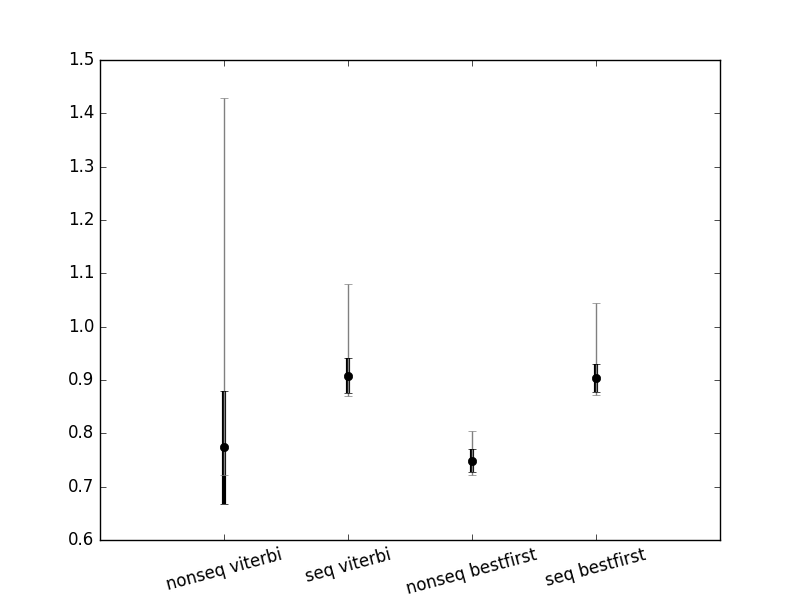
\includegraphics[width=0.90\linewidth]{fit_time.png}
	\label{fit-time}
	\caption{Czas uczenia (w ms)}
\end{figure}

\newpage

Kolejnym badaniem było sprawdzenie czasu testowania. Tutaj już widać znaczący, bo aż blisko 10-krotny wzrost czasu testowania zbioru sekwencyjnego względem zbioru bazowego. Różnice między algorytmami również nie są bardzo widoczne, zauważyć jednakże również można mniejszy rozrzut algorytmu \textit{best-first}.

\begin{table}[ht!]
\centering
\caption{Wyniki badań - czas testowania (w ms)}
\label{my-label}
\begin{tabular}{|c|c|c|c|c|}
\hline
\textbf{}     & \textbf{nonseq Viterbi} & \textbf{seq Viterbi} & \textbf{nonseq best-first} & \textbf{seq best-first} \\ \hline
\textbf{min}  & 0.1368                  & 1.1994               & 0.1366                     & 1.3415                  \\ \hline
\textbf{max}  & 0.2546                  & 1.7130               & 0.1640                     & 1.4338                  \\ \hline
\textbf{mean} & 0.1445                  & 1.2293               & 0.1418                     & 1.3628                  \\ \hline
\textbf{std}  & 0.0133                  & 0.0607               & 0.0050                     & 0.0157                  \\ \hline
\end{tabular}
\end{table}

\begin{figure}[h!]
	\centering
	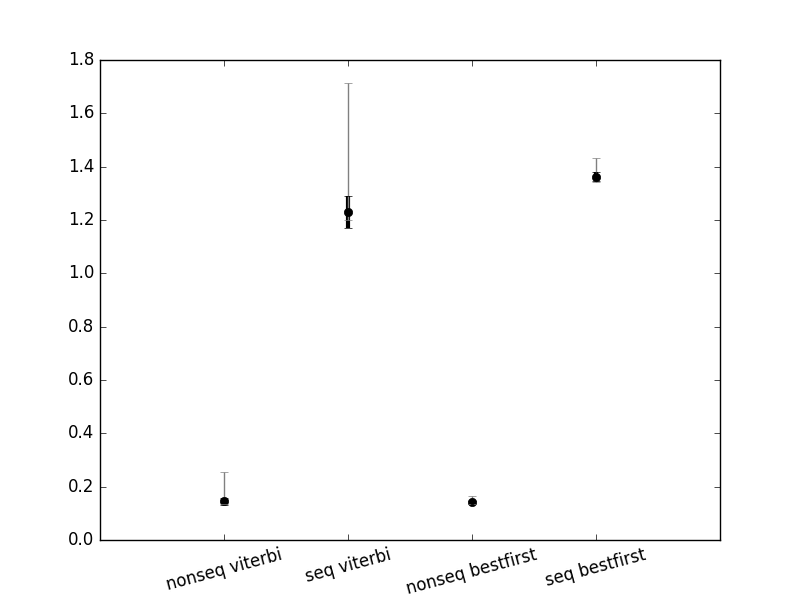
\includegraphics[width=0.90\linewidth]{score_time.png}
	\label{score-time}
	\caption{Czas testowania (w ms)}
\end{figure}

\newpage

Ostatnim przeprowadzonym eksperymentem było sprawdzenie efektywności modelu. Zauważyć można, iż na efektywność nie ma wpływu rodzaj zastosowanego zbioru, a wręcz zauważyć można, że dla zbioru sekwencyjnego rośnie rozrzut wartości względem zbioru bazowego, co sugeruje jego mniejszą stabilność. Różnice między dwoma algorytmami są także prawie niezauważalne.

\begin{table}[ht!]
\centering
\caption{Wyniki badań - dokładność (w \%)}
\label{my-label}
\begin{tabular}{|c|c|c|c|c|}
\hline
\textbf{}     & \textbf{nonseq Viterbi} & \textbf{seq Viterbi} & \textbf{nonseq best-first} & \textbf{seq best-first} \\ \hline
\textbf{min}  & 56.8965                 & 54.3859              & 56.8965                    & 45.6140                 \\ \hline
\textbf{max}  & 82.7586                 & 87.7192              & 82.7586                    & 86.8421                 \\ \hline
\textbf{mean} & 70.9827                 & 68.1140              & 70.2931                    & 68.2456                 \\ \hline
\textbf{std}  & 5.5390                  & 7.7356               & 5.0435                     & 9.6267                  \\ \hline
\end{tabular}
\end{table}

\begin{figure}[h!]
	\centering
	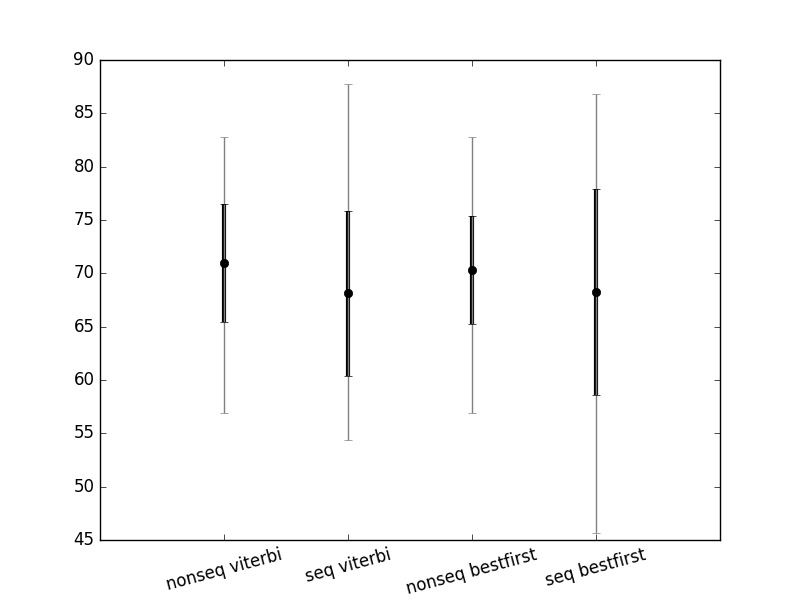
\includegraphics[width=0.90\linewidth]{accuracy.png}
	\label{accuracy}
	\caption{Dokładność (w \%)}
\end{figure}
